\documentclass[10pt]{article}

\usepackage{lipsum}
\usepackage{url}
\usepackage{float}
\usepackage{amsmath}
\usepackage{enumitem}
\usepackage{graphicx}
\usepackage{caption}
\usepackage{subcaption}
\usepackage{rotating}
\usepackage{geometry}
\usepackage{listings}
\usepackage{hyperref}
\usepackage[T1]{fontenc}
\usepackage[numbered]{matlab-prettifier}
\usepackage{siunitx}

\newcommand{\documentTitle}{Lab 3 - Basic Circuits}
\newcommand{\documentAuthor}{Andrew Pham, Aneel Damaraju}
\newcommand{\courseTitle}{ELEC 240}
\newcommand{\testDate}{September 19,2018}
\newcommand{\reportDate}{September 26, 2018}

\geometry{margin=1in}
\lstset{
    tabsize=4,
    basicstyle={\ttfamily},
    captionpos=b,
    belowskip=1em,
    aboveskip=1em,
    numbers=left,
	escapechar=\@,
}

\title{
    \textbf{\courseTitle} \\
    \textbf{\documentTitle} \\
    \bigskip
    \textbf{\large{Test performed: \testDate}} \\
    \textbf{\large{Report submitted: \reportDate}} \\
    \bigskip
    \bigskip
}
\author{\documentAuthor}
\date{}

\begin{document}

\maketitle

\newpage

\section{Objective}

In this lab, we explored Kirchoff's laws, and transfer functions through the use of various circuit elements, such as potentiometers, and software, such as LT Spice.

\medskip
In the first section of this lab, we explored running various amounts of AC and DC current through a voltage divider of different voltages. We also used a potentiometer as a voltage divider and verified its accuracy. In the second portion of this lab, we measured the transfer function of an RC Circuit by measuring its phase and amplitude with various input frequencies, and we then compared it with the calculated transfer function generated using MATLAB. Finally, we simulated two different RC circuits using LTSpice software and plotted the gain of the circuit at various input frequencies. 

%\textit{Note (To be deleted): Think of this test report as a document with your peers as your readers. This means you can assume a similar knowledge background as you. Your readers should be able to easily understand what is going on, and also be able to repeat your lab results based on your document and all references you cite.}

%\textit{For the Objective section, identify the test you performed and its objectives. The objectives of the test are important to state because they are usually analyzed in the conclusion to determine whether the test succeeded.}

\section{Materials}

\begin{itemize}
	\item Virtual Bench (Software, Oscilloscope, Function Generator, DC Power Supply)
	\item Computer with LTSpice Software 
	\item BNC Male to Clips cord
	\item BNC T connector
	\item Oscilloscope Probe
	\item Breadboard
	\item 2 10 cm length wires (with 6 mm stripped on each end)
	\item Digital Multimeter
	\item 10$k\Omega$ potentiometer
	\item 2 47$\Omega$ resistors
	\item 2 1$M\Omega$ resistors
	\item 2.2 $k\Omega$ resistor
	\item 2.2$\mu F$ resistor
	
\end{itemize}

\medskip

%\textit{Note (To be deleted): Provide a bullet point list of components, software tools, and hardware (such as the NI VirtualBench or DMM) used during the lab}

\section{Test Description}
In Part A of Experiment 3.1, we explored the freuqency range that the DMM on the Virtual Bench could usefully measure by outputting a sine wave from the function generator and recording the maximum voltage recorded by the DMM hooked up to this outputted sine wave. In Part B, we measured the output of a voltage divider and observed how circuits in reality deviate from ideal circuits. In Part C, we used a poteniometer as a voltage divider and verified that turning the slider in equal increments would proportionally increase the resistance of the potentiometer. 

In Part A of Experiment 3.2, we measured the transfer function of an RC Circuit that we wired on the breadboard by inputting various AC frequencies and measuring and plotting the resulting voltage signal. In Part B, we simulated an RC circuit by creating a virtual circuit on LTSpice. We then performed AC analysis by plotting the gain of the RC Circuit over a wide frequency range.  


\medskip

%\textit{Note (To be deleted): This section provides a summary of the test your team performed. Give enough information so readers can understand what you did, but do not go into the details of every step.}

\subsection{Pre-Lab Calculations and Schematics}

No pre-lab calculations were needed, but an understanding of how to measure a transfer function of an AC circuit was needed. Depicted below in Fig. \ref{measurement} is the desired oscilloscope output overlay needed to measure the transfer function:
\begin{centering}
	\begin{figure} [H]
		\centering
		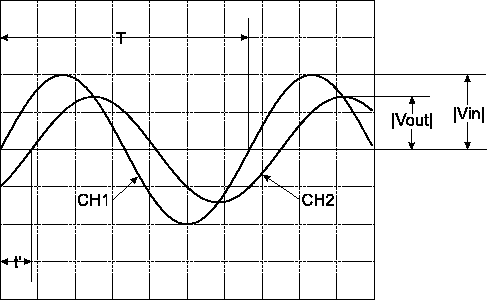
\includegraphics[scale=0.5]{images/measurementexample.png}
		\caption{Circuit Output Signal Overlayed with Function Generator Output}
		\label{measurement}
	\end{figure}
\end{centering}

To measure the transfer function at a given frequency, we needed to measure both $|V_{IN}|$ and $|V_{OUT}|$, which was achieved by measuring the height of the peaks of CH1 and CH2. To measure the phase $\Phi$, we measured the horizontal distance between the peaks of CH1 and CH2. With this technique, we are able to perform AC circuit analysis in Part A of Experiment 3.2. 
\medskip

%\textit{Note (To be deleted): Include the homework pre-calculations and schematics that serve as the initial setup for the test. Briefly explain the importance of each item you include. You may want to number your equations/figures so you can refer to them in later sections. Including photos of handwritten work is okay.}

\section{Results and Discussion}

\subsection{Experiment 3.1: Resistive Voltage Dividers}
\subsubsection{Part A}

	 The voltage reading on the DMM by a 2$V_{pp}$ sine wave is $.704 V_{rms}$, or .704 $V_{in}$. The voltage reading on the DMM for a similar square wave is 1.096 $V_{in}$. Then, readings were done for various frequencies for the same value sine wave as used in the initial test. The results were as follows
	\begin{table}[H]
		\begin{center}
			\caption{Voltage read by the DMM of the Sine Wave at given frequencies}
			\label{tab: 31A}
			\begin{tabular}{l|r}
				\textbf{Frequency} & \textbf{Voltage}\\
				(Hz) & (V)\\
				\hline
				5 & .641\\
				50 & .701\\
				500 & .701\\
				5k & .49\\
				50k & .0\\
			\end{tabular}
		\end{center}
	\end{table}
	It seems that the appropriate frequency for the DMM is 50-500 Hz to be safe, but more reasonably 10Hz-1kHz.
\subsubsection{Part B}
	 The voltage divider ratio should be $\frac{10}{10+10} = \frac{1}{2} V_{in}$  for two \SI{10}{\kilo\ohm} Resistors in series. For the sine wave, the output is $.351 V_{ac}$, which is 49\% of the initial Voltage, consistent with the voltage divider equation 
	 At 47 Ohms the $V_{out} = .243$, which is inconsistent, with the voltage divider equation, indicating that the voltmeter may have inconsistent readings at low voltages. 
	 At 1 MOhms the output voltage is .335, indicating that there may be a range of acceptable resistance for the voltmeter, just like we noted an acceptable frequency range.
\subsubsection{Part C} 
	Using the same sine wave, but wih 100 Hz, the potentiometer is connected in series and the voltage drop across it is recorded. At the midpoint, $V_{out} = .386 or .55 V_{in}$ this value is reasonable within error for such an analog device. 
	 The voltage divider ratio should be $\frac{10}{(10+10)}$  for two 10 kOhm Resistors in series. For the sine wave, the output is $.351 V_{AC}$, which is 49\% of the initial Voltage, consistent with the voltage divider equation 
	 At 47 Ohms the $V_{OUT} = .243$, which is inconsistent, with the voltage divider equation, indicating that the voltmeter may have inconsistent readings at low voltages. 
	 At 1MOhm the output voltage is .335, indicating that there may be a range of acceptable resistance for the voltmeter, just like we noted an acceptable frequency range.
\subsubsection{Part C} 
	Using the same sine wave, but wih 100 Hz, the potentiometer is connected in series and the voltage drop across it is recorded. At the midpoint, $V_{OUT} = .386 or .55 V_{IN}$ this value is reasonable within error for such an analog device. 
	The values of the output voltage at different divisions are given below.
\begin{table}[H]
	\begin{center}
		\caption{Voltage Across the Potentiometer at Each Division}
		\label{tab: 31C}
		\begin{tabular}{l|r}
			\textbf{Division} & \textbf{Voltage}\\
			(\#) & (V)\\
			\hline
			1 & .76\\
			2 & .653\\
			3 & .589\\
			4 & .506\\
			5 & .389\\
			6 & .273\\
			7 & .181\\
			8 & .076\\
			9 & .002\\
			10 & 0.0\\
		\end{tabular}
	\end{center}
\end{table}
 	It seems as if the values were evenly spaced as if they're were only 9 divisions, since the 9th and 10th both had 0V out.
\subsection{Experiment 3.2: Filters and Transfer Function}
\subsubsection{Part A}
	Measuring the frequency and the amplitude of the output voltage across an RC circuit. The values recorded can be seen below
\begin{table}[H]
\begin{center}
	\caption{Frequency and the amplitude of the output voltage across an RC circuit}
	\label{tab: 32A}
	   \begin{tabular}{l|c|r}
		\textbf{Frequency} & \textbf{Voltage} & \textbf{Phase shift}\\
		(Hz) & (V) & (ms) \\
		\hline
		20 & .99 & 1.97\\
		50 & .96 & 1.02\\
		100 & .88 & .869\\
		200 & .68 & .632\\
		500 & .39 & .402\\
		1k & .16 & .227\\
		2k & .065 & .119\\
		5k & .041 & .046\\
		10k & .021 & .023\\
		20k & .010 & .012\\
	\end{tabular}
\end{center}
\end{table}
\begin{center}
	\begin{figure} [H]
		\centering
		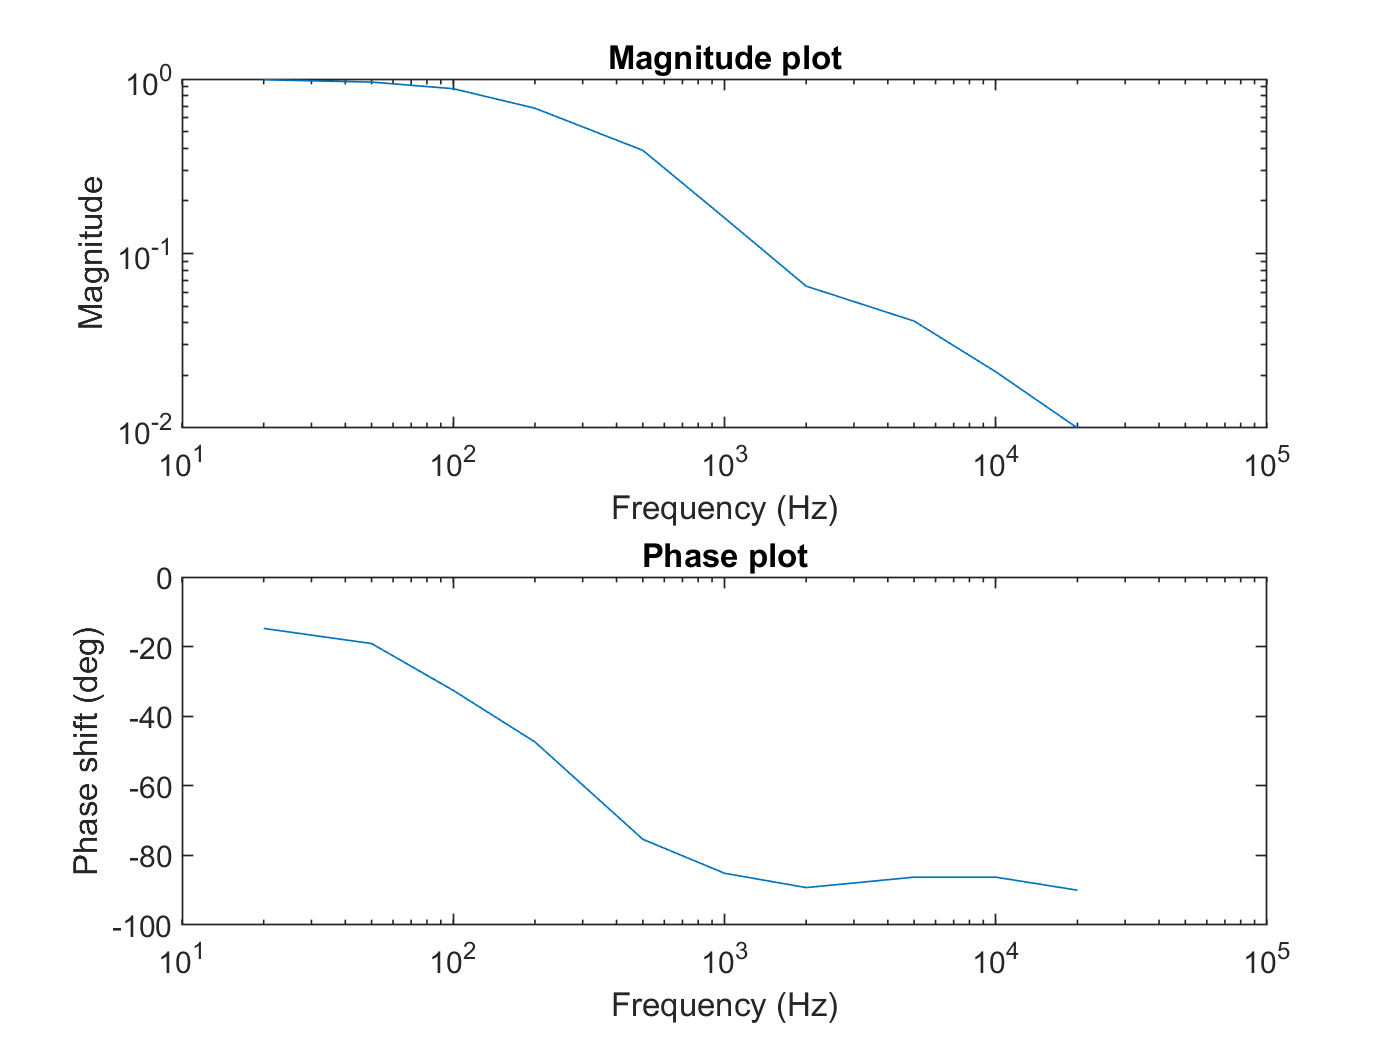
\includegraphics[scale=0.4]{images/ourRC.png}
		\caption{Visualization of the magnitude and phase plots for table \ref{tab: 32A}}
		\label{fig:32A5}
	\end{figure}
\end{center}
\begin{center}
	\begin{figure} [H]
		\centering
		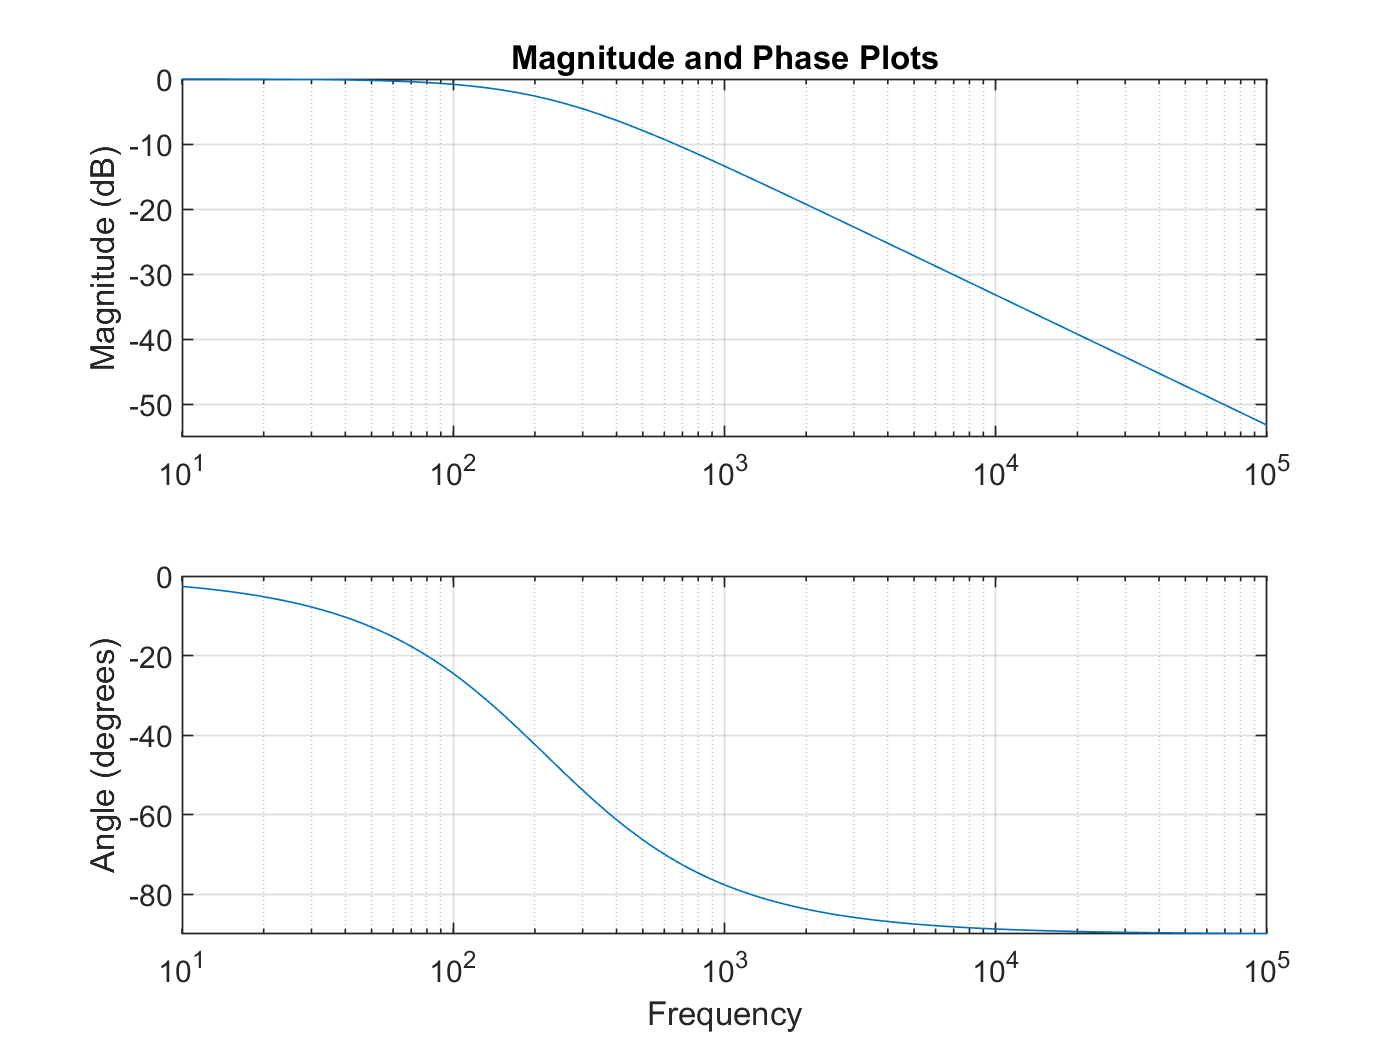
\includegraphics[scale=0.4]{images/matlabRC.png}
		\caption{Using the given transfer function, used the supplied magphase function to generate the expected values}
		\label{fig:32A6}
	\end{figure}
\end{center}
These results from Table \ref{tab: 32A} were then used plotted onto Figure \ref{fig:32A5}, using MATLAB. When compared to the values of Figure \ref{fig:32A6} it can be seen that the experimental results match up with the calculated results, confirming the transfer function of $\frac{1}{RCj2\pi f+1}$, where $R = \SI{2.2}{\kilo\ohm}$ and $C = \SI{.33}{\mu\farad}$. The experimental results, while scattered, are confirmed by the theoretical results. 

\subsubsection{Part B}
\begin{center}
	\begin{figure} [H]
		\centering
		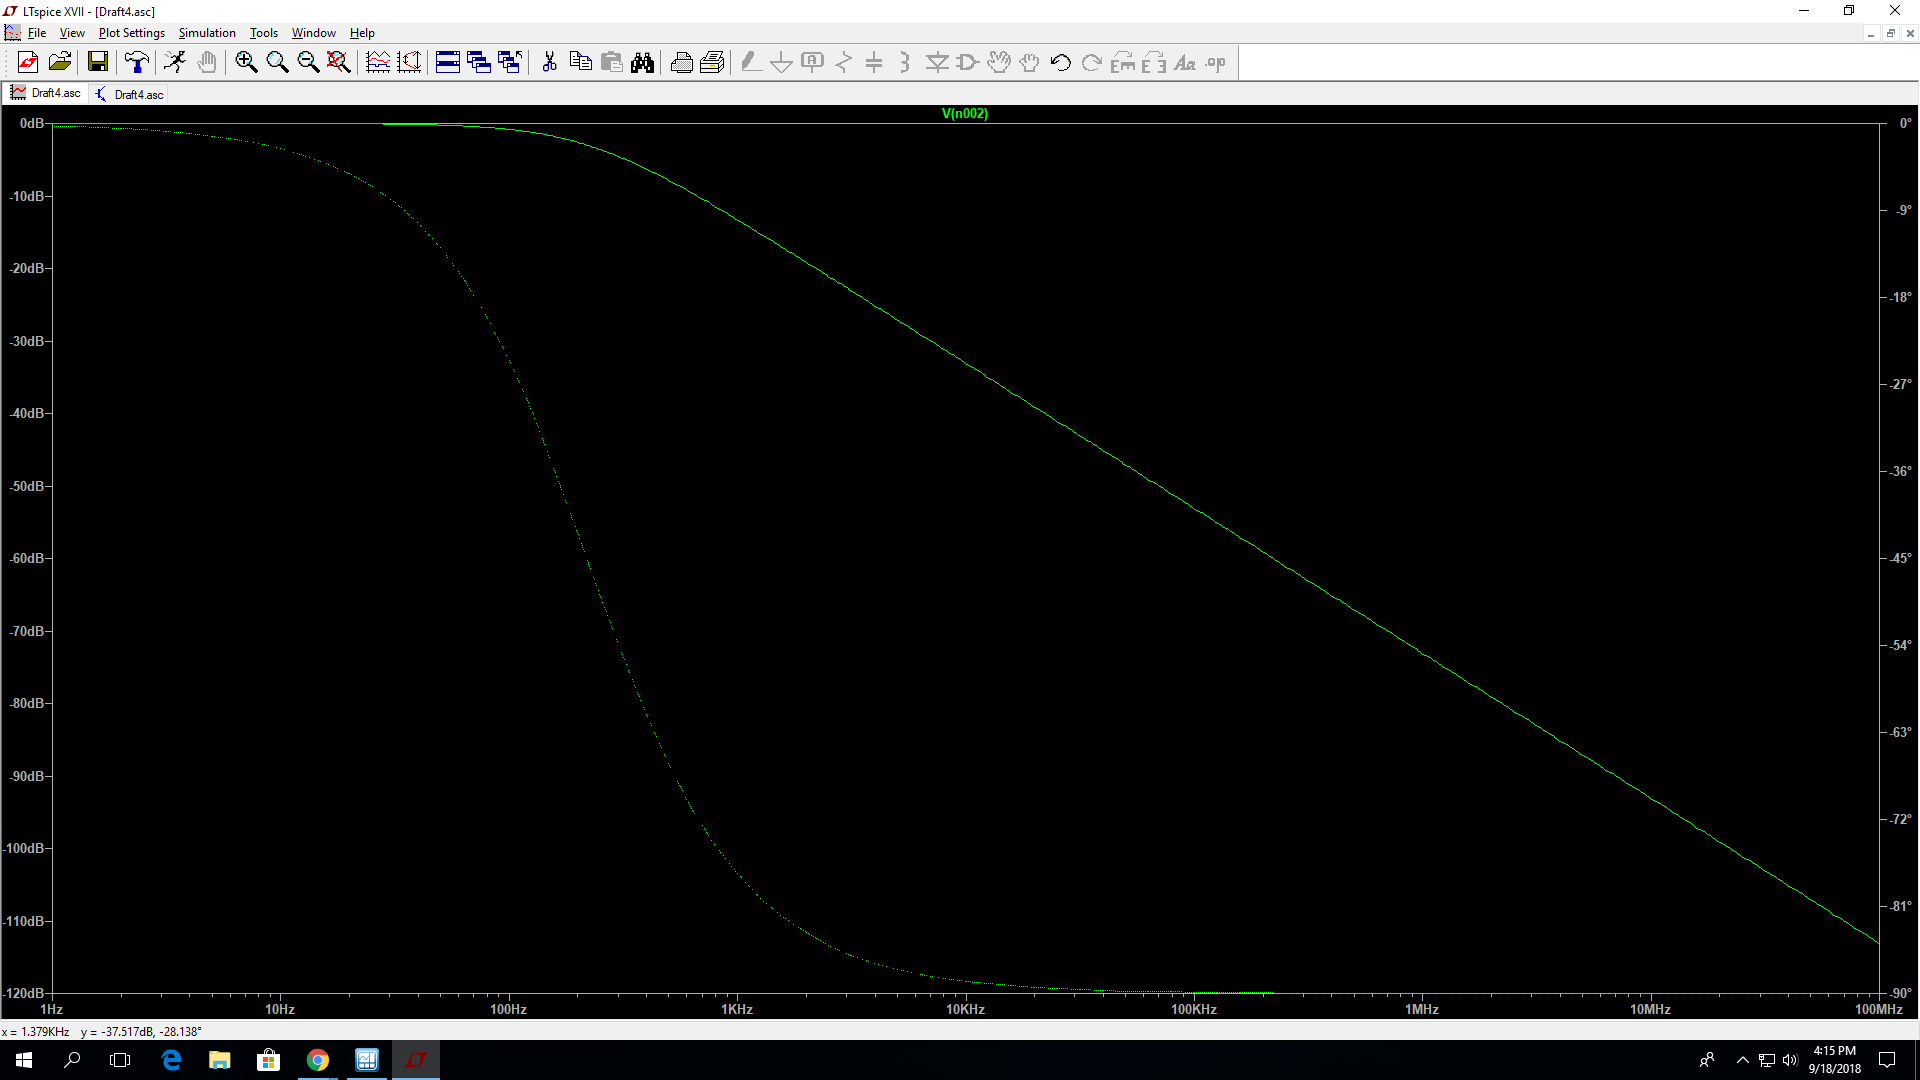
\includegraphics[scale=0.22]{images/simple.png}
		\caption{LT Spice AC analysis of simple RC circuit built in lab, as observed, it is a low pass filter}
		\label{fig:simpleRC}
	\end{figure}
\end{center}
The screenshot of the LT spice AC analysis of an RC circuit can be seen in figure \ref{fig:simpleRC}, The gain at low frequencies is 0 dB or 1 V/V. The cutoff frequency happens at approx. 220 Hz. At high frequencies the gain rolloff becomes almost linear, with a slope of -1 dB/dec. At low frequencies, the phase is $0^\circ$ or in phase. At high frequencies the phase is $-90^\circ$. This is because a capacitor will ideally lag in voltage when put in a circuit in series, and at low frequencies the capacitor acts more like a resistor.
\begin{center}
	\begin{figure} [H]
		\centering
		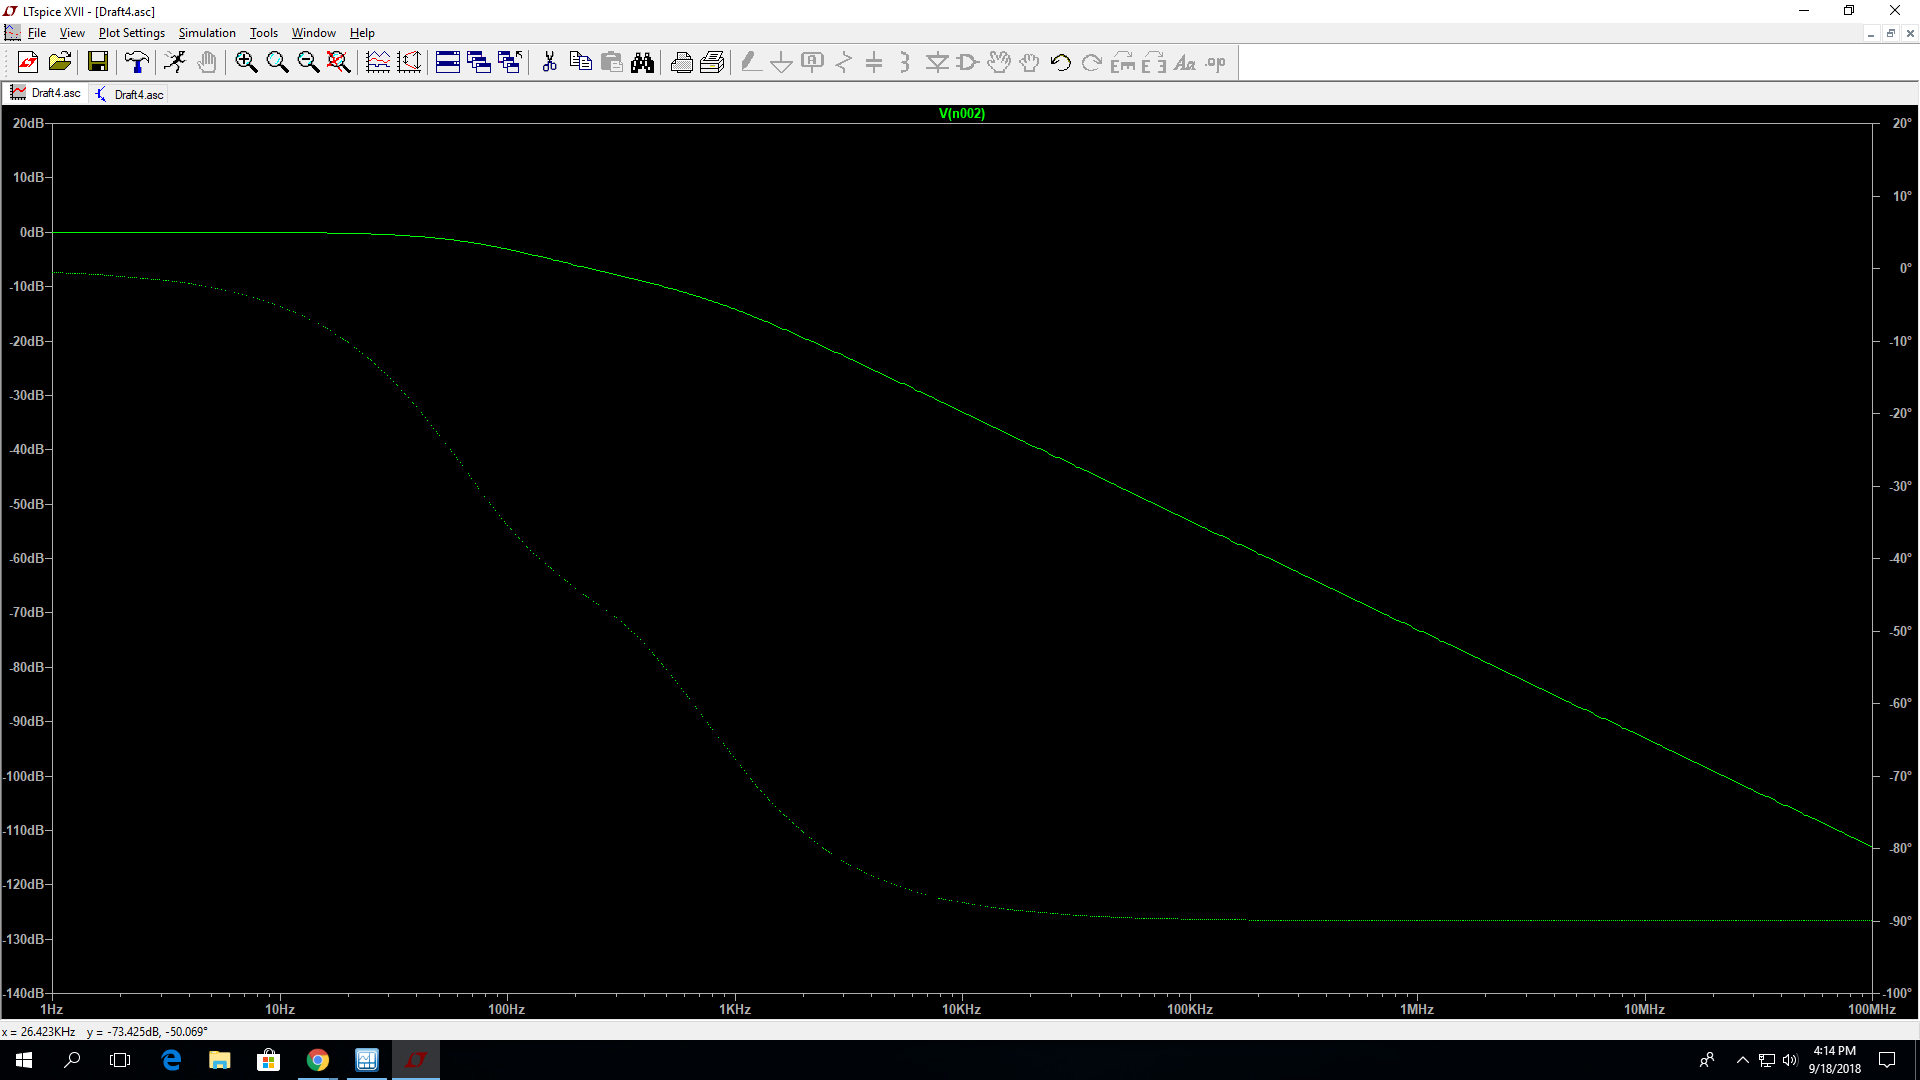
\includegraphics[scale=0.22]{images/cascade.png}
		\caption{LT Spice AC analysis of the combination RC circuit. It is a low pass filter, but slightly more complex, due to the cascading RC element}
		\label{fig:cascading}
	\end{figure}
\end{center}
After adding the cascading RC circuit, the graph looks a little more interesting, including 2 bumps but a similar DC gain, as seen in Figure \ref{fig:cascading}. However, the cutoff frequency is approximately the same as before. The gain rolloff has changed, and in this case, it seems to have the same slope, maybe around -1 dB/dec. While the phase at high frequencies is 90$^\circ$, the DC phase is around 8$^\circ$. Cascading two identical filters can allow the phase to shift, even for low frequencies while keeping the cutoff frequency approximately the same.


\section{References}

\begin{itemize}
	\item https://www.ece.rice.edu/~dpr2/elec240/lab3
\end{itemize}

\medskip

%\textit{Note (To be deleted): List any datasheets, websites, lab procedure, etc. used during the lab.}

\section{Conclusion}
In Part A of Experiment 3.1, we discovered that the useful frequency range of the digital multimeter was roughly 50-500Hz. We hypothesize that this limited frequency rate is due to the physical limitations of the multimeter in how fast it can read the signal; too fast a frequency, the DMM will not be able to fully record the waveform. \\ In Part B of the same experiment, we found that the voltmeter also has a limited voltage range that it can accurately measure. We received different values for $V_{OUT}$ for a 47$\Omega$ resistor and a 1$M\Omega$ resistor. We believe that this discrepancy arises from the fact that the voltmeter has a finite internal resistance; when measuring voltage through lower resistor values, this finite internal resistance of the voltmeter will appreciably affect the voltage measurement.  \\In Part C, we measured a 10$k\Omega$ potentiometer's resistance at its ten predefined intervals to see if the equation $V_{OUT} = \alpha V{IN}$ was correct, where $\alpha$ was a constant that corresponded to a fraction of $V_{IN}$ (i.e. $\alpha = 1$ means $V_{OUT} = 0.1V_{IN}$. This is assumption is mostly correct according to the data we recorded in Table \ref{tab: 31C}; however, we noticed that $V_{OUT}$ was essentially zero by the time we set the slider to the 9th position. This may have been due to a slight miscalibration in the potentionometer itself. \\\\
In Part A of Experiment 3.2, we used the measurement techniques from the pre-lab section to measure the transfer function of a simple RC circuit that we built from a 2.2$k\Omega$ resistor and a 0.33$\mu F$ capacitor. We found that the measured magnitude and phase plots looked almost exactly like the MATLAB plots that we generated by entering the transfer function $\frac{1}{RCj2\pi f+1}$ into the \textit{magphase} function. These results validate both our  measuring techniques and the calculated transfer function. \\ In Part B of the same experiment, we used LTSpice to simulate a simple and a slightly more complex RC circuit to observe their various properties. For the simple RC circuit, we found that the rolloff of the gain is approximately 1 dB/dec. We also found that the phase of the RC circuit dropped much more quickly than the gain as frequency increased, going from $0^\circ$ at 1 Hz to nearly $-90^\circ$ at 100 kHz. This lag at high frequencies reflects the presence of a capacitor, which acts like a resistor at low frequencies (which do not cause phase shift) but causes high phase shifts at higher frequencies (capacitors take the derivative of voltage, which phase shifts by $-90^\circ$ by changing a sine to a cosine). We observed a similar magnitude plot for the more complex cascading RC circuit. However, we did note a difference in the phase plot, which had a brief bump around 500 kHz where it would be linear in the simpler RC circuit. Furthermore, the DC phase shift was approximately $8^\circ$. Thus, we conclude that putting RC circuits in cascade will maintain the cutoff frequency and the magnitude plot of the transfer function but will shift the phase plot. 

%\textit{Note (To be deleted): While the ``Results and Discussion'' section focused on the test results individually, the ``Conclusion'' discusses the results in the context of the entire experiment. Usually, the objectives given in the ``Introduction'' are reviewed to determine whether the experiment succeeded. If the objectives were not met, you should analyze why the results were not as predicted.}

\section{Errors}
\begin{itemize}
	\item \textit{Did not receive a ratio of $V_{IN}/V_{OUT}=0.5$ for the 47 $\Omega$ resistor}: This is due to the fact that the voltmeter has a finite internal resistance. When a low resistance value is being measured, the effects of this finite internal resistance become higher. 
	\item \textit{Voltmeter recorded a $V_{OUT}$ of 0 for division \#9}: This error is likely due to a miscalibration in the potentiometer that caused it to reach its maximum resistance slightly before the 10th turn of the slider knob. 
\end{itemize}
%Your text here

\medskip

%\textit{Note (To be deleted): Briefly list sources of error and discuss how to eliminate or deal with them}

\end{document}
